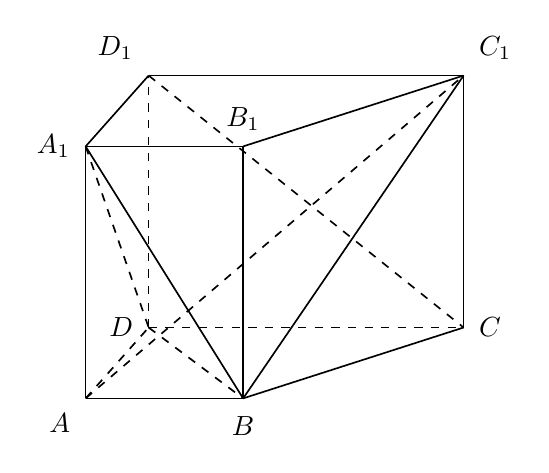
\begin{tikzpicture}[line width=0.6pt, >=stealth]
% Oblique schematic of right quadrangular prism ABCD-A1B1C1D1
\coordinate (A) at (0,0);
\coordinate (B) at (2,0);
\coordinate (D) at (0.8,0.9);
\coordinate (C) at (4.8000000000,0.9000000000);
\coordinate (A1) at (0,3.2);
\coordinate (B1) at (2,3.2);
\coordinate (D1) at (0.8,4.1);
\coordinate (C1) at (4.8000000000,4.1000000000);
% visible prism edges
\draw (A) -- (A1);
\draw (A) -- (B);
\draw (B) -- (C);
\draw (B) -- (B1);
\draw (C) -- (C1);
\draw (A1) -- (B1);
\draw (B1) -- (C1);
\draw (C1) -- (D1);
\draw (D1) -- (A1);
\draw (A1) -- (B);
\draw (B) -- (C1);
% hidden edges
\draw[dashed] (A) -- (D);
\draw[dashed] (D) -- (C);
\draw[dashed] (D) -- (D1);
\draw[dashed] (A1) -- (D);
\draw[dashed] (D) -- (B);
\draw[dashed] (A)--(C1);
\draw[dashed] (D1)--(C);
% labels offset from strokes
\node[below left=2pt] at (A) {$A$};
\node[below=3pt] at (B) {$B$};
\node[right=2pt] at (C) {$C$};
\node[left=2pt] at (D) {$D$};
\node[left=2pt] at (A1) {$A_{1}$};
\node[above=2pt] at (B1) {$B_{1}$};
\node[above left=2pt] at (D1) {$D_{1}$};
\node[above right=2pt] at (C1) {$C_{1}$};
\end{tikzpicture}
